\documentclass[12pt]{article}

\usepackage[document]{ragged2e}
% Math package
\usepackage{amsmath}

% Math symbols (like Laplace operator)
\usepackage{mathrsfs}

% Geometry package for setting margins
\usepackage{geometry}
% Set margins
\geometry{margin=1in}

% Color package for highlighting text and array columns
\usepackage[table]{xcolor}

% Command \T now inserts a bold math t (for convenience)
\newcommand{\T}{\mathbf{t}}
% Command \F now inserts a bold math f (for convenience)
\newcommand{\F}{\mathbf{f}}

% Package for sans-serif font
\usepackage{helvet}
\renewcommand{\familydefault}{\sfdefault}

% ---
% Setting math font to sans-serif

% \usepackage[cm]{sfmath}
% \usepackage{cmbright}

% \usepackage{arev}

% \usepackage{fontspec}
% \setmathrm{Arial}
% \setmathsf{Arial}
% \setmathtt{Arial}
% \setboldmathrm[BoldFont={Optima ExtraBlack}]{Optima Bold}
% ---

% Package for the Aboxed command
\usepackage{mathtools}

% Package for creating equations side-by-side
\usepackage{multicol}

% Package for adding space between paragraphs
\usepackage{parskip}

% Package for changing enumerate letters
\usepackage{enumitem}

% \dd for typesetting differentials
\usepackage{physics}

% Adding "Page {number} of {total}" in footer
\usepackage{lastpage}
\usepackage{fancyhdr}
\fancyfoot[C]{Page \thepage\ of {\hypersetup{linkcolor=black}\pageref{LastPage}}}
\pagestyle{fancy}
% Remove horizontal line from header
\renewcommand{\headrulewidth}{0pt}
\setlength{\headheight}{15pt}

% I'm more used to typing \infin for infinity symbol :P
\newcommand*{\infin}{\infty}

% Colors
\usepackage{xcolor}
\definecolor{codegreen}{rgb}{0,0.6,0}
\definecolor{codegray}{rgb}{0.5,0.5,0.5}
\definecolor{codepurple}{rgb}{0.58,0,0.82}
% \definecolor{backcolour}{RGB}{211,211,211}
\definecolor{backcolour}{rgb}{0.92,0.92,0.92}
\definecolor{rulecolour}{rgb}{0.5,0.5,0.5}
% \definecolor{backcolour}{rgb}{0.95,0.95,0.92}

% For code blocks
\usepackage{listings}

\definecolor{javared}{rgb}{0.6,0,0} % for strings
\definecolor{javagreen}{rgb}{0.25,0.5,0.35} % for comments
\definecolor{javapurple}{rgb}{0.5,0,0.35} % for keywords
\definecolor{javadocblue}{rgb}{0.25, 0.35, 0.75} % for javadoc

\lstdefinestyle{javastyle}{
    language=Java,
    basicstyle=\ttfamily\footnotesize,
    keywordstyle=\color{javapurple}\bfseries,
    stringstyle=\color{javared},
    commentstyle=\color{javagreen}\itshape,
    morecomment=[s][\color{javadocblue}]{/**}{*/},
    numbers=left,
    numberstyle=\tiny\color{gray},
    stepnumber=1,
    numbersep=10pt,
    backgroundcolor=\color{white},
    showspaces=false,
    showstringspaces=false,
    showtabs=false,
    frame=single,
    tabsize=4,
    captionpos=b,
    breaklines=true,
    breakatwhitespace=true,
    % escapeinside={\%*}{*)},
}

% Package for diagonal fractions
\usepackage{xfrac}

% Floating images
\usepackage{float}

% Subfigure images
\usepackage{subcaption}

% Making the "Figure #" bold in figures
\usepackage[labelfont=bf]{caption}

% Hyperlinks
\usepackage{hyperref}
\hypersetup{
    colorlinks,
    citecolor=black
    % filecolor=black,
    % linkcolor=black,
    % urlcolor=black
}

% SI units
\usepackage{siunitx}

% Table styles
\usepackage{booktabs}

% Typing derivatives
\usepackage{esdiff}

% Fill table of contents lines with dots
\usepackage{tocloft}
\renewcommand{\cftsecleader}{\cftdotfill{\cftdotsep}}

% Appendix package
\usepackage[title, titletoc]{appendix}

% Making the title look nice
\usepackage{titling}

\newcommand*{\dif}{\mathrm{d}}
\newcommand*{\dt}{\mathop{\mathrm{d}t}}
\newcommand*{\im}{\mathrm{j}}
\newcommand*{\cosx}[1]{\cos \left( #1 \right)}
\newcommand*{\sinx}[1]{\sin \left( #1 \right)}

% Laplace transform operator
\newcommand*{\Laplace}[1]{\mathscr{L} \left\{ #1 \right\}}
\newcommand*{\ILaplace}[1]{\mathscr{L}^{-1} \left\{ #1 \right\}}

% Inline code
% \newcommand*{\code}[1]{{\fontfamily{lmtt}\fontseries{b}\selectfont #1}}

\usepackage{tikz}
\usepackage{eso-pic}
\usepackage{xcolor}
\usepackage{setspace}

% Packages for custom inline code style
\usepackage[skins]{tcolorbox}
\usepackage{etoolbox}
\usepackage{soul}

\definecolor{MyRed}{HTML}{e90c2f}

\newcommand{\AddRedStripe}{
  \AddToShipoutPictureBG*{%
    \AtPageUpperLeft{%
      \begin{tikzpicture}[remember picture, overlay]
        % Adjust these coordinates to move the stripe
        \fill[MyRed] ([yshift=-8cm]current page.north west) rectangle ([yshift=-13cm]current page.north east);
      \end{tikzpicture}%
    }%
  }
}

\newcommand*{\sk}{

    \vspace{\baselineskip}

}

\begin{document}

    % Custom inline code style
    \newtcbox{\code}{on line,
        colback=gray!15, colframe=gray!80,
        boxrule=0.4pt, arc=2pt,
        top=0.1em, bottom=0.1em, left=0.3em, right=0.3em,
        fontupper=\ttfamily\footnotesize,
        box align=base, sharp corners,
        enhanced, 
    }

%     \newcommand{\code}[1]{%
%     \begingroup
%     \lstinline[backgroundcolor=\color{gray!15},basicstyle=\ttfamily\small]{#1}%
%     \endgroup
%   }

    \newgeometry{left=1.3in, right=1.3in}
    \newlength\myheight
    \newlength\mydepth
    \settototalheight\myheight{Xygp}
    \settodepth\mydepth{Xygp}
    \setlength\fboxsep{0pt}
    \setlength{\fboxrule}{0pt}
    \begin{titlepage}
        \AddRedStripe
        \vspace*{-1.5cm}
        \Huge\textbf{EECS 4313}

        \LARGE \textbf{Software Engineering Testing}

        \Large\textbf{Final Project Report --- Testing Thumbnailator}

        \Large April 7, 2025

        \vspace{1.4cm}

        \begin{figure}[H]
            \centering
            
\includegraphics[width=0.95\textwidth]{images/york-lassonde-logos.drawio.png}
        \end{figure}

        % \vspace{1.9cm}
        \vfill

        \normalsize

        \begin{spacing}{0.5}
            \textbf{Group F}
            \sk

            Isaiah Gocool

            goisaiah@my.yorku.ca

            218918052

            \sk
            \sk

            Mher Eric Gyulumyan

            mericg@my.yorku.ca

            217990540

            \sk
            \sk

            Daniel Di Giovanni

            dand02@my.yorku.ca

            218204818
        \end{spacing}

        \normalsize
        \begin{center}
            \rule{\textwidth}{1pt}\\
        \end{center}


    \end{titlepage}

    \setlength\fboxsep{5pt}
    \setlength{\fboxrule}{1pt}
    \restoregeometry

    \pagenumbering{roman}

    {\hypersetup{linkcolor=black}
        \tableofcontents
        \thispagestyle{plain}
    }

    \pagebreak

    \pagenumbering{arabic}

    \section{Introduction}
    \markboth{}{}

    Testing is an essential component of the software development lifecycle,
        ensuring that code behaves as expected and meets specified requirements.
    By systematically validating the functionality and performance of a program,
        testing helps uncover hidden bugs, improve reliability, and facilitate
        future maintenance.
    Robust testing practices are particularly important in environments where
        software quality and stability are paramount, such as in production
        systems and mission-critical applications.

    This project involved analyzing and testing an existing software project
        called Thumbnailator.
    Thumbnailator is an open-source Java library designed to simplify the
        creation of image thumbnails with minimal setup and external
        dependencies.
    Specifically, two classes in the Thumbnailator library will be tested here:
        \code{ThumbnailatorUtils.java} and \code{BufferedImageBuilder.java}.

    In addition to traditional test design, this report incorporates the use of
        generative AI tools to enhance test case generation, increase code
        coverage, and analyze potential faults or refactoring opportunities.
    Coverage metrics are measured using JaCoCo (Miller's metric), with a focus
        on achieving near-complete line and branch coverage.

    The remainder of this report details the chosen testing techniques,
        justifies their application to individual methods, documents any bugs or
        refactoring suggestions, and evaluates coverage results.
    All tests are implemented using JUnit 5 and are located in the src/test/java
        directory of the project.

    \section{Testing Methods}
    \markboth{}{}

    The testing methods for each of the two classes will be presented here, as
        well as their results.

    \subsection{ThumbnailatorUtils.java}
    \markboth{}{}

    The \code{ThumbnailatorUtils} class is a final utility class within the
        Thumbnailator library that provides static methods for querying
        supported image output formats and compression types.
    It acts as a lightweight wrapper around the Java ImageIO API, offering
        convenience methods for checking format availability and compatibility
        with specific compression types.
    These functions play a key role in determining how images are saved and
        encoded, making their correctness essential for the reliable generation
        of thumbnails.

    \subsubsection{Equivalence Class Testing for ThumbnailatorUtils.java}
    \markboth{}{}

    For the testing of the ThumbnailatorUtils class, Equivalence Class Testing
        was selected as the primary technique.
    This method was well-suited for the nature of the class, which consists of
        utility functions that operate on clearly defined inputs and produce
        predictable, categorized outputs.
    Each method in this class is deterministic, and the expected outcomes can be
        effectively grouped into equivalence classes. For example, valid
        versus invalid image format strings, supported versus unsupported
        compression types, and null versus non-null return values from the
        underlying ImageIO API.

    We applied a robust equivalence class testing approach to ensure that both
        valid and invalid inputs were covered.
    For methods that accepted a single input parameter, such as
        \code{getSupportedOutputFormats()} and
        \code{isSupportedOutputFormat(String format)}, we used the weak robust
        method, selecting one valid and one or more invalid values to test
        boundary and error-handling behavior.
    In contrast, for methods accepting multiple parameters, such as
        \code{isSupportedOutputFormatType(String format, String type)}, we
        applied strong robust equivalence testing to evaluate all combinations
        of valid and invalid inputs, ensuring thorough interaction coverage
        between the parameters.

    Overall, equivalence class testing was an efficient and logical choice for
        this class because it allowed us to validate functional correctness
        across the full behavioral spectrum while minimizing redundant or
        low-value test cases.
    The clear structure and deterministic behavior of these methods made them
        ideal candidates for this technique.

    \markboth{}{}
    \subsubsection{Weaknesses of Equivalence Class Testing ThumbnailatorUtils.java}
    \markboth{}{}

    While equivalence class testing proved to be an effective technique for
        covering a wide range of expected behaviors, it does have limitations in
        this context.
    One of the key drawbacks is that it does not inherently account for internal
        control flow or edge cases within complex logic branches.
    For example, the method\\
    \code{isSupportedOutputFormatType(String format, String type)} contains
        multiple conditional paths, some of which are tightly coupled with
        constants like \code{ORIGINAL\_FORMAT} and\\
        \code{DEFAULT\_FORMAT\_TYPE}.
    Although equivalence class tests can verify correctness for typical input
        scenarios, they may miss subtle bugs hidden in rare or unusual paths
        unless specifically targeted.

    Furthermore, this technique assumes that inputs within the same equivalence
        class will result in the same output behavior, which may not always be
        the case in methods that interact with external libraries like ImageIO.
    These dependencies can introduce inconsistencies depending on platform
        support or registry state, potentially causing false confidence if not
        supplemented with additional testing methods.
    In such cases, more granular structural techniques, like path testing or
        decision coverage, might be necessary to ensure that all control paths
        have been exercised.

    Despite these limitations, equivalence class testing still offered strong
        value in efficiently validating the public-facing functionality of ThumbnailatorUtils. However, in a production environment, it would be advisable to complement it with more exhaustive white-box techniques for maximum reliability.

    \markboth{}{}
    \fancyhead{}
    \subsection{BufferedImageBuilder.java}
    \markboth{}{}

    The \code{BufferedImageBuilder.java} class is a utility designed to simplify the
        construction of BufferedImage objects in Java.
    It provides multiple constructors and method chains that allow clients to
        configure the width, height, and image type of the image to be created.
    Internally, it applies validation to ensure that dimensions are positive and
        handles specific cases like substituting unsupported image types (e.g.,
        \code{BufferedImage.TYPE\_CUSTOM}) with safe defaults.
    The \code{build()} method is responsible for returning a new image instance
        with the specified attributes.
    The class is central to how images are generated in a controlled and
        reusable way within the Thumbnailator library.

    \markboth{}{}
    \subsubsection{Equivalence Class Testing for BufferedImageBuilder.java}
    \markboth{}{}

    To test this class, Equivalence Class Testing was selected as the primary
        technique.
    This method was an ideal fit given that the class operates on a finite and
        well-defined set of input parameters: integer values for width, height,
        and image type.
    These inputs naturally form logical groups of valid and invalid values,
        allowing us to define equivalence classes such as positive dimensions
        versus zero or negative values, and supported image types versus special
        or custom types.

    We used a robust equivalence class testing approach to ensure input
        validation was thoroughly exercised.
    For constructors and methods that accepted single inputs, such as
        \code{width(int)} and \code{height(int)}, we employed weak robust
        equivalence classes, validating representative valid values
        (e.g., 1, 100) and invalid ones (e.g., 0, -5).
    For constructors or methods involving multiple parameters, such as\\
        \code{(int width, int height, int imageType)}, we used strong robust
        equivalence testing, evaluating combinations of valid and invalid
        values across each parameter to ensure defensive programming logic was
        correctly enforced.

    This approach enabled us to systematically verify the builder's correctness
        and input validation across both constructor-based and method-chained
        object creation paths without exhaustive testing of the inputs.
    The class's tight scope and clear validation logic made it highly compatible
        with this technique.

    \markboth{}{}
    \subsubsection{Weaknesses of Equivalence Class Testing BufferedImageBuilder.java}
    \markboth{}{}

    However, equivalence class testing has its limitations.
    It does not provide direct insight into internal control flow or ensure
        coverage of every possible execution path.
    For example, while we tested input classes that trigger validation logic,
        equivalence class testing does not guarantee that all edge-case
        interactions between methods like \code{width()}, \code{height()}, and
        \code{imageType()} have been fully explored unless explicitly designed
        for.
    Additionally, this technique assumes uniform behavior across members of the
        same class, but if unexpected branching or undocumented behavior were
        present, they could potentially go undetected.

    Despite these limitations, equivalence class testing offered a structured
        and focused strategy for verifying the functionality of
        \code{BufferedImageBuilder}.
    The class's clear parameter constraints and straightforward behavior made it
        an ideal candidate for this technique.
    In a more complex system, this approach would benefit from being
        supplemented by structure-based techniques such as decision or condition
        coverage to ensure complete control flow validation.

    \markboth{}{}
    \section{Testing Results}
    \markboth{}{}

    This section explains the results of testing both the
        \code{ThumbnailatorUtils.java} and\\
        \code{BufferedImageBuilder.java}
        classes, as well as suggestions for improvement.

    \markboth{}{}
    \subsection{Testing Results of ThumbnailatorUtils.java}
    \markboth{}{}

    All of the test cases we made for the \code{ThumbnailatorUtils.java} class
        are passing, as shown in the IntelliJ screenshot in Figure
        \ref{fig:thumnailator_utils_test_results}.
    \begin{figure}[H]
        \centering
        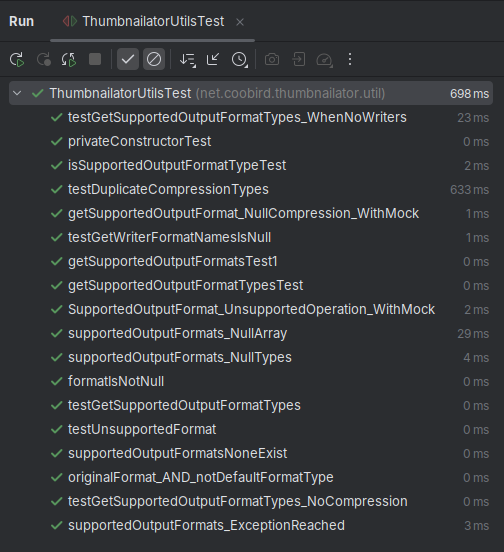
\includegraphics[width=0.6\textwidth]{images/thumnailator_utils_test_results.png}
        \caption[All test cases passing for ThumbnailatorUtils.java.]{All test cases passing for ThumbnailatorUtils.java.}
        \label{fig:thumnailator_utils_test_results}
    \end{figure}
    No faults were discovered during testing of the ThumbnailatorUtils class.
    The test suite effectively covered all public methods and validated expected
        behavior across a wide range of input combinations.
    Code coverage analysis using JaCoCo reported 96\% line and
        branch coverage.

    Upon inspection of the coverage report, the uncovered branch was found in a
        conditional check that is unreachable by design.
    This code section is shown below in Listing \ref{lst:impossibe_coverage}.
    The second condition of the second branch (\code{type != ThumbnailParameter.DEFAULT\_FORMAT\_TYPE })
        did not get fully tested, as shown in the JaCoCo screenshot in Figure
        \ref{fig:jacoco_impossible_coverage}.

    \lstinputlisting[style=javastyle,caption={Code section that did not achieve 100\% coverage.},label=lst:impossibe_coverage,captionpos=b]{code/ImpossibleCoverage.java}

    \begin{figure}[H]
        \centering
        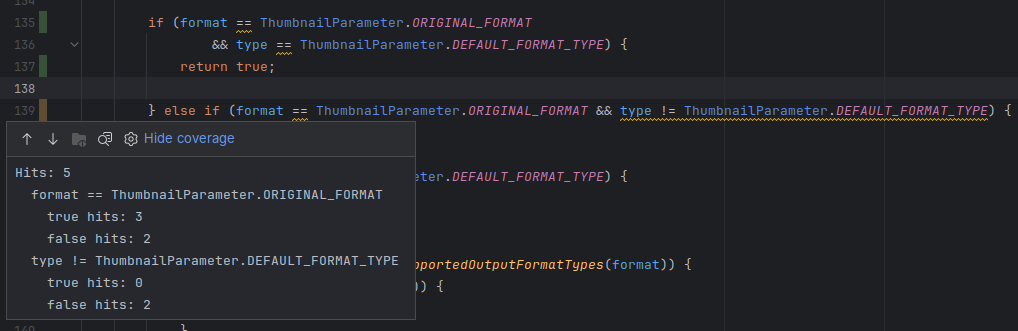
\includegraphics[width=0.95\textwidth]{images/jacoco_impossible_coverage.png}
        \caption[JaCoCo feedback of untested conditional branch.]{JaCoCo feedback of untested conditional branch.}
        \label{fig:jacoco_impossible_coverage}
    \end{figure}

    To aid in analysis, we simplify the code as shown in Listing
        \ref{lst:simplified_impossibe_coverage}, where \code{A} represents the
        condition \code{format == ThumbnailParameter.ORIGINAL\_FORMAT} and
        \code{B} represents the condition
        \code{type == ThumbnailParameter.DEFAULT\_FORMAT\_TYPE}.

    \lstinputlisting[style=javastyle,caption={Simplified code analysis of Listing \ref{lst:impossibe_coverage}.},label=lst:simplified_impossibe_coverage,captionpos=b]{code/SimplifiedImpossibleCoverage.java}

    There are four possibilities for the values of \code{A} and \code{B}:
    \begin{enumerate}
        \item
            \code{A = T, B = T}:
                First branch evaluates to true and is taken, the rest of the
                    conditional block is untested.
        \item
            \code{A = T, B = F}:
                First branch evaluates to false second branch evaluates to true,
                    so both \code{A} and \code{!B} are tested in the second
                    branch.
        \item
            \code{A = F, B = T}:
                Both the first and second branches evaluate to false by
                    short-circuiting on the first condition, which means the
                    second condition of the second branch (\code{!B}) does not
                    get tested.
        \item
            \code{A = F, B = F}:
                Both the first and second branches evaluate to false by
                    short-circuiting on the first condition, which means the
                    second condition of the second branch (\code{!B}) does not
                    get tested.
    \end{enumerate}
    As such, due to the structure of this conditional block and the
        short-circuiting behavior of Java conditional expressions, the second
        condition of the second statement will never be tested in the negative
        (when \code{!B = F}).

    This highlights an opportunity for refactoring, which is discussed in the
        next section.

    \markboth{}{}
    \subsection{Refactoring Suggestions for ThumbnailatorUtils.java}
    \markboth{}{}

    Although no functional faults were found in \code{ThumbnailatorUtils.java},
        code coverage analysis and inspection revealed areas that could benefit
        from refactoring to improve clarity and testability.
    These suggestions are also available as formal bug reports in Appendices
        \ref{sec:appendix_a} and \ref{sec:appendix_b}.

    \subsubsection{Redundant Conditions}

    In the method
        \code{isSupportedOutputFormatType(String format, String type)}, as shown
        in \ref{lst:impossibe_coverage}, the conditional block contains
        redundant and unreachable logic.
    By refactoring the code as shown in Listing \ref{lst:possibe_coverage}, the
        clarity is improved and 100\% code coverage is possible.

    \lstinputlisting[style=javastyle,caption={Rafctoring suggestion of Listing \ref{lst:impossibe_coverage} for improved clarity and code coverage.},label=lst:possibe_coverage,captionpos=b]{code/PossibleCoverage.java}

    \subsubsection{Non-Null API Assumption}

    In the method \code{getSupportedOutputFormats()}, the following logic checks
        for a \code{null} return from \code{ImageIO.getWriterFormatNames()}, as
        shown in Listing \ref{lst:image_io_null}.

    \lstinputlisting[style=javastyle,caption={Redundant null checks for ImageIO library.},label=lst:image_io_null,captionpos=b]{code/ImageIONull.java}

    According to the official Java documentation and observed runtime
        behavior,\\
        \code{ImageIO.getWriterFormatNames()} never returns \code{null}.
    Instead, it returns an empty array if no formats are found.
    The \code{null} check can only be tested through mocking, which introduces
        artificiality into test scenarios.
    Removing this condition (or replacing it with a check for an empty array)
        would simplify the logic and reduce reliance on mocks to achieve full
        coverage.
    This is shown in Listing \ref{lst:image_io_not_null}.

    \lstinputlisting[style=javastyle,caption={Refactored-out null checks for ImageIO library.},label=lst:image_io_not_null,captionpos=b]{code/ImageIONotNul.java}

    By addressing these areas, the codebase can be slightly streamlined without impacting functionality, while also improving maintainability and correspondence between tests and actual runtime behavior.

    \markboth{}{}
    \subsection{Testing Results of BufferedImageBuilder.java}
    \markboth{}{}

    All of the test cases we made for the \code{BufferedImageBuilder.java} class
        are passing, as shown in the IntelliJ screenshot in Figure
        \ref{fig:buffered_image_builder_test_results}.
    \begin{figure}[H]
        \centering
        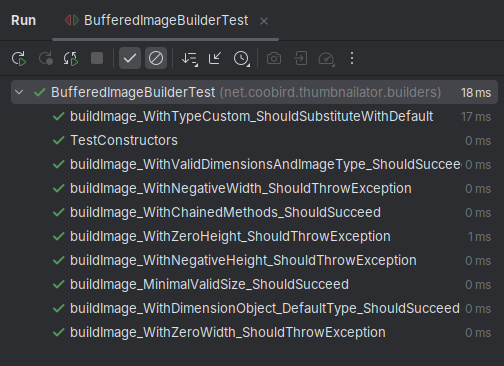
\includegraphics[width=0.6\textwidth]{images/buffered_image_builder_test_results.png}
        \caption[All test cases passing for BufferedImageBuilder.java.]{All test cases passing for BufferedImageBuilder.java.}
        \label{fig:buffered_image_builder_test_results}
    \end{figure}

    No refactoring was deemed necessary for the \code{BufferedImageBuilder.java}
        class.
    This class adheres well to the Single Responsibility Principle, with its
        sole purpose being the creation of \code{BufferedImage} instances based
        on configurable parameters.
    The class design is straightforward, with clear constructor overloads and
        method chains for setting width, height, and image type.
    Input validation is explicitly handled through concise checks with
        informative exception messages, and the \code{build()} method reliably
        encapsulates object creation.

    Given its focused scope, minimal complexity, and high readability, the class
        is already well-structured and easy to test.
    All logic paths are meaningful and reachable, and coverage was easily
        brought to 100\% without requiring mocking or workaround
        strategies.
    As such, no structural or stylistic changes are recommended.

    \section{Use of Generative AI}
    \markboth{}{}

    Generative AI tools were incorporated throughout the testing process to
        improve coverage quality, identify refactoring opportunities, and
        streamline test development.
    These tools were used in a complementary role to human analysis, helping
        both accelerate and validate the design of the test suite.

    \markboth{}{}
    \subsection{AI Assistance for ThumbnailatorUtils.java}
    \markboth{}{}

    For the \code{ThumbnailatorUtils.java} class, AI tools were primarily used
        to apply more comprehensive coverage testing methods.
    Specifically, we consulted AI to explore advanced usage patterns of Mockito,
        including static mocking via \code{MockedStatic}, which was essential
        for simulating edge cases related to the ImageIO API.
    We were also advised by the AI tool to upgrade our Mockito dependency to
        version 4.11.0 and add the Mockito-inline version 4.11.0 dependency for
        static mocks.
    This guidance allowed us to test behavior that would otherwise be
        unreachable using standard input values alone, such as
        \code{ImageIO.getWriterFormatNames()} returning null, or mocked
        \code{ImageWriter} instances throwing
        \code{UnsupportedOperationException}.

    Additionally, AI was used for providing refactoring suggestions based on
        unreachable branches identified through coverage analysis.
    After sharing specific blocks of logic, the tool helped confirm that certain
        conditions (e.g., unreachable branches in\\
        \code{isSupportedOutputFormatType}) were redundant and could be
        simplified.
    This aided in creating a more concise and maintainable version of the logic
        without altering functionality.

    \markboth{}{}
    \subsection{AI Assistance for BufferedImageBuilder.java}
    \markboth{}{}

    In the case of \code{BufferedImageBuilder.java}, AI was used for automated
        test case generation.
    After analyzing the class structure and its parameter constraints, we used
        AI to outline equivalence classes and generate a corresponding set of
        JUnit test cases.
    These included valid and invalid inputs for dimensions, special cases like
        \code{TYPE\_CUSTOM}, and boundary conditions such as minimal valid size
        (1x1).
    This significantly accelerated the test writing process while ensuring
        methodical and consistent coverage across all input categories.

    By using generative AI as a development partner, we were able to improve the
        efficiency, coverage, and depth of our testing effort, particularly in
        areas involving external dependencies and low-level control validation.
    This approach also ensured alignment with modern best practices in
        test-driven development and code quality assurance.

    \section{Conclusion}

    This report presented a comprehensive testing approach for two classes in
        the Thumbnailator library: \code{ThumbnailatorUtils.java} and
        \code{BufferedImageBuilder.java}, as assigned to Group F.

    Using equivalence class testing as the primary method, we systematically
        identified and validated input-output behaviors across all relevant
        functional paths.
    For BufferedImageBuilder, testing resulted in 100\% line and
        branch coverage, with no faults discovered and no need for refactoring.
    The class's simplicity, clear responsibilities, and input validation made it
        ideal for this type of testing.
    For \code{ThumbnailatorUtils.java}, testing achieved 96\%
        coverage, with all functional paths validated except for one unreachable
        branch.
    This led to targeted refactoring suggestions aimed at improving clarity and
        reducing dead code.

    Generative AI tools were used strategically to enhance the testing process,
        from assisting in advanced Mockito usage and identifying refactoring
        opportunities to helping generate automated test cases for complex
        equivalence classes.
    These tools significantly improved testing depth and efficiency,
        particularly for edge cases involving external dependencies.

    Overall, the testing strategies applied to both classes demonstrated a high
        level of coverage and confidence in correctness, while also showcasing
        the value of combining structured testing techniques with modern
        AI-assisted workflows.

    \pagebreak

    \vspace*{5cm}
    \part*{Appendices}
    \addcontentsline{toc}{part}{Appendices}
    \thispagestyle{empty}
    \pagebreak

    \begin{appendices}
        \markboth{}{}
        \section{Bug Report for isSupportedOutputFormatType Method of ThumbnailatorUtils Class}
        \label{sec:appendix_a}
        \markboth{}{}
        \begin{center}
            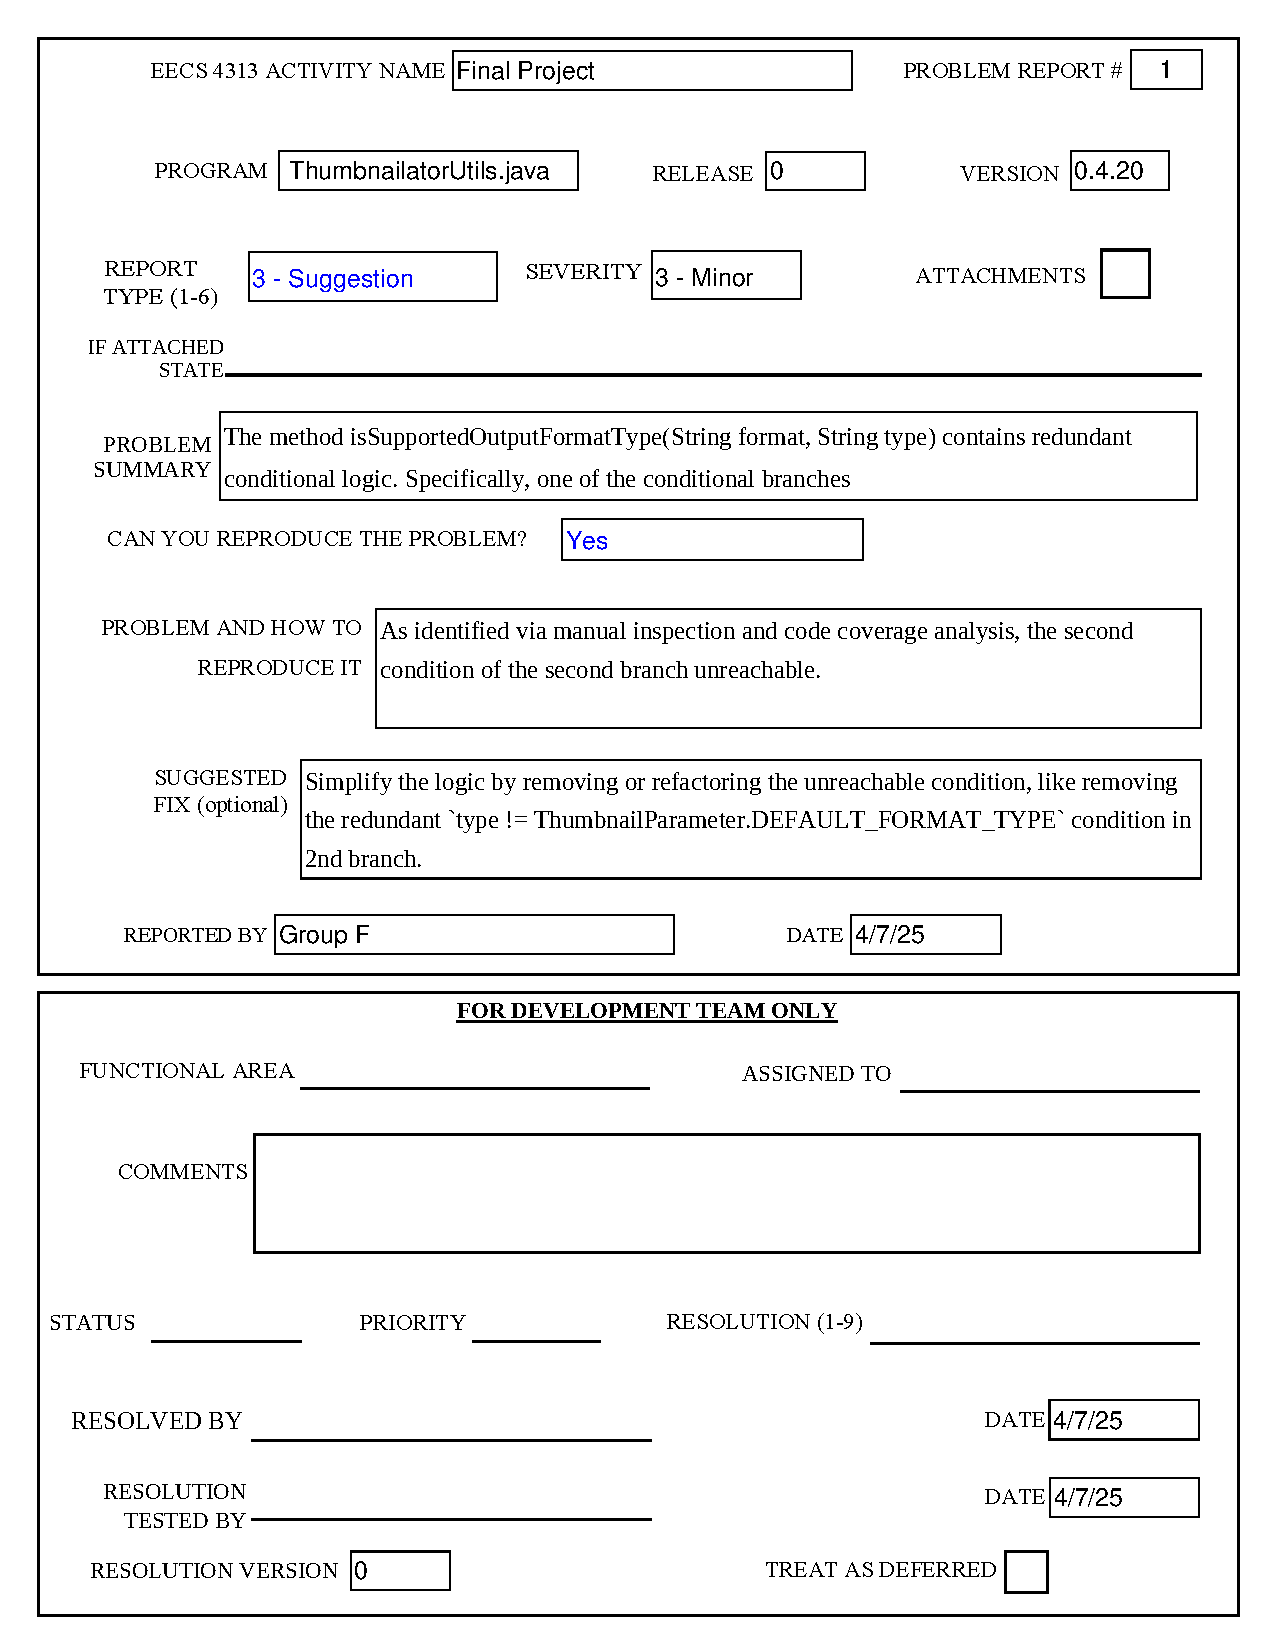
\includegraphics[width=0.9\textwidth]{bug_reports/Bug_Report_1_print.pdf}
        \end{center}

        \markboth{}{}
        \section{Bug Report for getSupportedOutputFormats Method of ThumbnailatorUtils Class}
        \label{sec:appendix_b}
        \markboth{}{}
        \begin{center}
            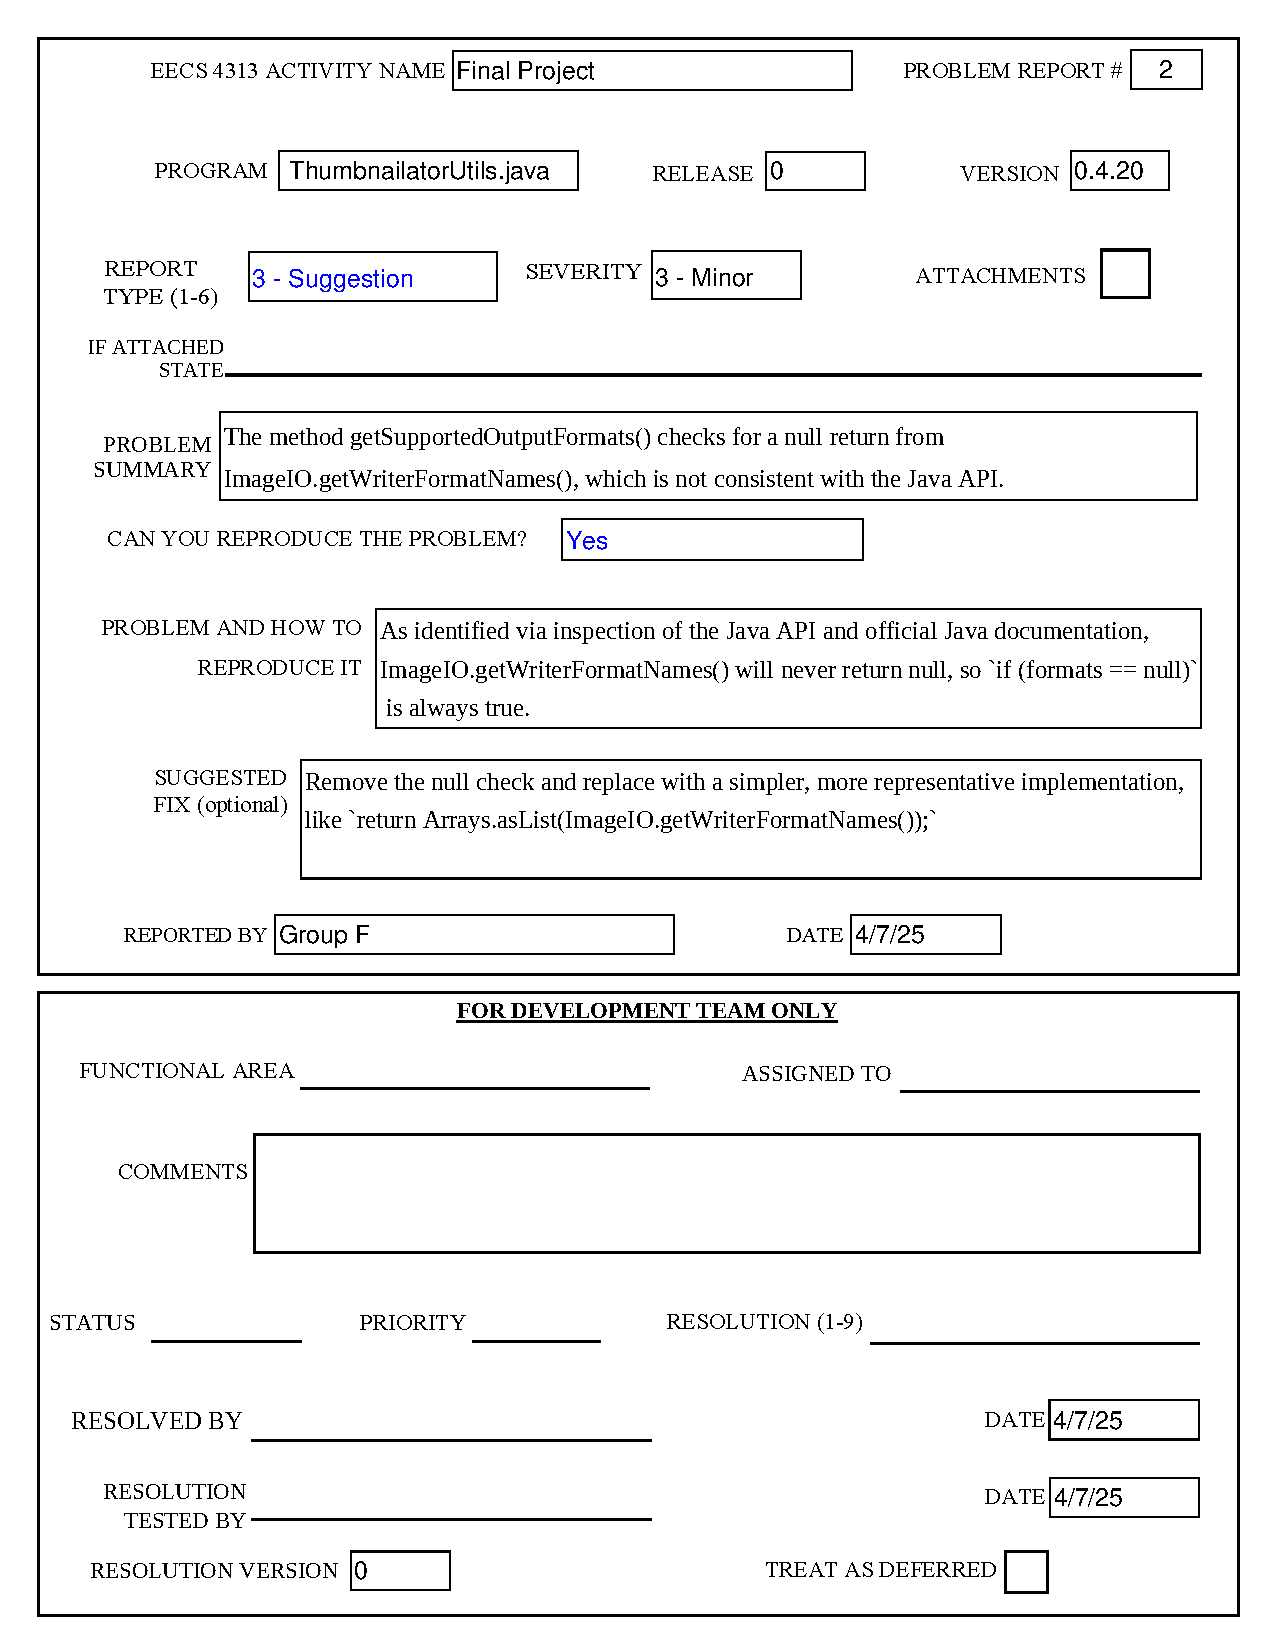
\includegraphics[width=0.9\textwidth]{bug_reports/Bug_Report_2_print.pdf}
        \end{center}
    \end{appendices}

\end{document}
